\documentclass[12pt]{article}
\usepackage[a4paper, margin=.30in]{geometry}
\usepackage{graphicx ,
            wrapfig,
            xcolor, 
            enumerate,
            amsmath,fontenc
            }

\newcommand\headerMe[2]{\noindent{}#1\hfill#2}
\renewcommand{\thesection}{\Roman{section}}

\author{Zakaria HAOUZAN}
\date{\today}

\begin{document}
% headers --------------
\headerMe{Matière : Physique-Chimie}{Professeur : Zakaria HAOUZAN}\\
\headerMe{Unité : Introduction }{Établissement : Lycée SKHOR qualifiant}\\
\headerMe{Niveau : 2BAC-SM-X}{Heure : 2H}\\

% ------Content ________
\begin{center}

    \Large{Leçon $N^{\circ} 1 $: \color{red} Questions qui se posent au physicien  }
\end{center}

%\begin{wrapfigure}[10]{r}{0.5\textwidth}
%    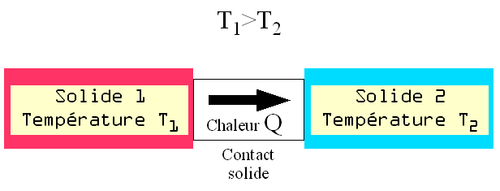
\includegraphics[width=0.5\textwidth]{./img/img00.png}
%\end{wrapfigure}
\section{ La Physique :}
La physique est une science qui s'intéresse à l'étude et à l'explication des phénomènes naturels et universels et leurs
évolutions dans l'espace et dans le temps. Elle établit des théories et des lois qui permettent
de les modéliser et de les prévoir.

\section{ Quelques activités du physicien : }

Le physicien observe et étudie les phénomènes naturels et universels tout en cherchant les lois qui les gouvernent.Il
fait des recherches théoriques et expérimentales pour approfondir la connaissance des phénomènes étudiés et mettre
au point de nouvelles méthodes et de nouveaux appareils en contribuant par ses recherches à l'évolution des sciences.

\section{Les questions que se posent les physiciens: }
Plusieurs questions peuvent se poser sur un physicien dans le but de comprendre le fonctionnement des phénomènes
parmi lesquelles on peut citer:
\begin{itemize}
   \item Quelles sont les grandeurs qui permettent d'étudier l'évolution du système étudié ?
   \item Quelles sont les paramètres extérieurs qui commandent cette évolution ?
   \item L'évolution étudiée peut-elle être caractériser par un ou plusieurs temps caractéristique?
   \item Quelle est le rôle des conditions initiales dans l'évolution du système étudié ?
   \item L'évolution étudiée est elle lente, rapide, totale ou limitée , est elle uniforme ou variée? ....

\end{itemize}

      Ensuite le physicien invente des théories et des lois qui expliquent les phénomènes observés tout en se basant sur
l'observation en passant par l'utilisation d'un modèle théorique ou expérimental avant d'extraire les résultats .

Par exemple c'est l'observation de la chute d'une pomme (d’un pommier) qui a conduit Newton à la découverte de la
lois d'attraction universelle.
Newton à son époque s’est posé plusieurs questions :
\begin{itemize}
   \item Qui fait tomber la pomme de l’arbre vers le sol ?
   \item Pourquoi la pomme ne s'éloigne de la terre à tout jamais.?
   \item Pourquoi la Lune ne tombe-t-elle pas elle aussi?
   \item la chute des corps et la révolution de la Lune autour de la terre, obéissent-elles à la même loi physique ?
      \end{itemize}
Ce qui a poussé Newton à découvrir la loi de gravitation universselle suivante:
Tous les corps s'attirent proportionnellement au produit de leurs masses et inversement porportionnelle au carré de la
distance qui les sépare.
\section{Rappel de quelques notions acquises utilisées dans les mesures effectuées par le physicien:}

\subsection{La longueur:}
\subsubsection{Unité de mesure de la longueur: }
L'unité de mesure de la longueur dans le système international est le mètre (m).
Les multiples et les sous multiples du mètre: (tableau de conversion)

\begin{center}
   \begin{tabular}{ |c|c|c|c|c|c|c| }
      \hline
      km & hm & dam & \bf{m} & dm & cm & mm \\
      \hline
        &   &    &  &   &   & \\
\hline
\end{tabular}
On place un seul nombre dans chaque case.
\end{center}
Exemple : 1m  =  100cm et 1cm = 0.01m = $10^{-2}$m

\underline{Autres unités de longueur:}

\begin{itemize}
   \item Le micromètre symbole $\mu$. $1\mu = 10^{-6} m$
   \item Le nonomètre symbole n. $1nm = 10^{-9} m$
   \item Le picomètre symbole p. $1pm = 10^{-12} m$
   \item -L’année lumière al : La distance parcourue par la lumière en une année.\\ $1al = c.\Delta{t} = 3.10^{8}.(365.25 . 24. 3600)= 9.5 10^{15}m$
\end{itemize}

\subsubsection{`Exemples de quelques longueurs :` Le périmètre d’un cercle de rayon R : $P = 2\pi.R$}

\section{La surface:}
\subsection{Unité de mesure de la surface: }
L'unité de mesure de la surface dans le système international est le mètre carré $(m^2)$.
Les multiples et les sous multiples du mètre carré: (tableau de conversion)

\begin{center}
   \begin{tabular}{ |c|c|c|c|c|c|c| }
      \hline
      $km^2$ & $hm^2$ & $dam^2$ & \bf{$m^2$} & $dm^2$ & $cm^2$ & $mm^2$ \\
      \hline
        &   &    &  &   &   & \\
\hline
\end{tabular}
\end{center}
Exemple : $1m^2 = 10^4 cm^2$ et $1cm^2 = 0.0001m^2 = 10^{-4} m^2$


\subsection{Exemples de quelques sufaces:}
\begin{itemize}
   \item Surface d’un disque de rayon R: $S = \pi.R^2$
   \item Surface d’un rectangle S=a.b avec a: longeur , b :largeur
   \item -Surface d’un cylindre de rayon R et de hauteur h: (deux fois la surface de base + la surface latérale) $S = 2\pi.R^2 + 2\pi.R.h$
\end{itemize}
\section{volume:}
L'unité de mesure du volume dans le système international est le mètre cube (m3).
Les multiples et les sous multiples du mètre cube: (tableau de conversion)
\begin{center}
   \begin{tabular}{ |c|c|c|c|c|c|c| }
      \hline
      $km^3$ & $hm^3$ & $dam^3$ & \bf{$m^3$} & $dm^3$ & $cm^3$ & $mm^3$ \\
      \hline
        &   &    &  &   &   & \\
\hline
\end{tabular}
   \begin{tabular}{ |c|c|c|c|c|c| }
      \hline
       $hL$ & $daL$ & \bf{$L$} & $dL$ & $cL$ & $mL$ \\
      \hline
        &   &    &  &   &    \\
\hline
\end{tabular}
\end{center}

Exemple : $1m^3 = 10^6 cm^3$ et $1cm^3 =  10^{-6} m^3$

Remarque: Pour mesurer le volume des liquides on utlise souvent le litre symbolisé par (L)
Les multiples et les sous multiples du litre: (tableau de conversion)
\begin{center}

\end{center}

Exemple : $1m^3 = 10^3 $L et $1L =  1000 mL$ 



\end{document}

